\section{Method}
\label{sec:method}

This section introduces the overall architecture of ApproxDA, then describes the three controllable approximation operators used to reformulate the dual-attention module, and finally analyzes their computational complexity.

\subsection{Architecture Overview}

ApproxDA-TransUNet adopts the hybrid CNN--ViT encoder-decoder structure of DA-TransUNet~\cite{sun2024datransunet}, with an R50-ViT-B/16 backbone pretrained on ImageNet-21K. Three CNN encoder stages produce multi-scale features at strides 4, 8, and 16; a 12-layer ViT processes $14{\times}14$ patch tokens. ApproxDABlocks replace all dual-attention modules at three skip connections---512 channels at $28{\times}28$, 256 at $56{\times}56$, and 64 at $112{\times}112$---and at the bottleneck.

ApproxDA-TransUNet is designed around an explicit hypothesis: that three orthogonal approximation operators---windowed PAM, low-rank projection, and grouped CAM---can replace the quadratic DA module to yield both a practical efficient architecture and a systematic framework for studying when approximation is appropriate. Each operator targets a distinct approximation axis (spatial scope, representation fidelity, channel scope), so any two can be held fixed while the third varies. This makes ApproxDA not merely a faster model, but a model whose design enables controlled ablation of approximation effects across tasks with different contextual requirements.

\begin{figure}[t]
  \centering
  \fbox{\rule{0pt}{2.5cm}\rule{\columnwidth}{0pt}}
  \caption{ApproxDA-TransUNet architecture. ApproxDABlocks (Low-Rank Windowed PAM + Grouped CAM + gate routing) replace dual-attention modules at all skip connections and the bottleneck. \texttt{gate\_mode} controls the routing during ablation.}
  \label{fig:framework}
\end{figure}

Figure~\ref{fig:framework} illustrates the overall ApproxDA architecture.

\subsection{Attention Approximation Formulation}

The original DA module performs dense spatial and channel attention over the full feature map, with quadratic complexity in both spatial resolution and channel dimension. ApproxDA reduces this cost along three independent axes, each targeting a distinct aspect of the approximation:

\textbf{Spatial scope} (window size $M$) controls \emph{how far} PAM reaches. Full global attention ($M{=}H$) captures all long-range spatial relationships; restricting to $M{\times}M$ local windows trades long-range context for lower complexity. This axis most directly governs whether high-GCR tasks retain the anatomical context they require.

\textbf{Representation fidelity} (rank $r$) controls \emph{how precisely} attention is computed within each window. Low-rank projection ($r \ll M^2$) approximates the affinity matrix at reduced cost; higher $r$ approaches exact attention.

\textbf{Semantic interaction} (groups $G$) controls \emph{which channels} may interact in CAM. Partitioning $C$ channels into $G$ independent groups reduces cross-channel dependency while retaining within-group semantic interaction.

These axes correspond to three distinct types of approximation: \emph{spatial approximation} (how far attention reaches, controlled by $M$), \emph{representation approximation} (how precisely affinity is computed, controlled by $r$), and \emph{channel approximation} (how broadly channels interact, controlled by $G$). The axes are fully independent: any two of $\{M,\,r,\,G\}$ can be held fixed while the third varies, enabling clean ablations that isolate individual approximation effects. Figure~\ref{fig:approx_space} visualizes this three-dimensional approximation space.

\begin{figure}[t]
  \centering
  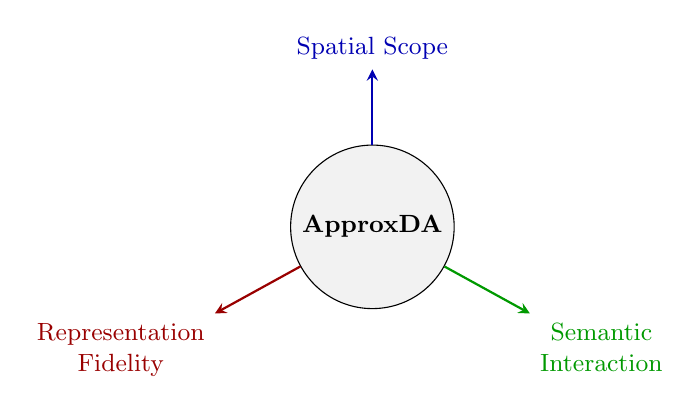
\begin{tikzpicture}[
    axis/.style={->, thick, >=stealth},
    lab/.style={font=\small, align=center}
  ]
    \node[draw, circle, fill=gray!10, minimum size=1.1cm, font=\small\bfseries] (c) at (0,0) {ApproxDA};
    \draw[axis, blue!70!black]  (c) -- ++(0, 2.0)
      node[lab, above] {Spatial Scope};
    \draw[axis, red!60!black]   (c) -- ++(-2.0,-1.1)
      node[lab, below left] {Representation\\Fidelity};
    \draw[axis, green!60!black] (c) -- ++(2.0,-1.1)
      node[lab, below right] {Semantic\\Interaction};
  \end{tikzpicture}
  \caption{ApproxDA's three-dimensional approximation space. Each axis is independently controllable. Spatial scope ($M$) most directly governs long-range context capture and thereby approximation effectiveness on high-GCR tasks.}
  \label{fig:approx_space}
\end{figure}

\subsection{Spatial Approximation}

Instead of computing global position attention, ApproxDA partitions the feature map into non-overlapping windows of size $M{\times}M$. Attention is computed independently inside each local window, reducing complexity from $\mathcal{O}(N^2C)$ to $\mathcal{O}(NM^2C)$.

\textbf{Window partitioning.} Following~\cite{liu2021swin}, we partition the feature map into $n_W$ non-overlapping $M{\times}M$ windows. Window clamping $M \leftarrow \min(M, H, W)$ allows $M{=}112$ to yield global attention at all scales, enabling a clean ablation that isolates windowing from low-rank as the performance bottleneck.

\textbf{Low-rank projection.} Following~\cite{wang2020linformer}, query and key features inside each window are projected from $N_w {=} M^2$ to rank $r \ll M^2$ via a learned matrix $\mathbf{W}_r \in \mathbb{R}^{r \times N_w}$:
\begin{equation}
  \tilde{\mathbf{C}} = \mathbf{W}_r \mathbf{C}^\top, \quad \tilde{\mathbf{D}} = \mathbf{W}_r \mathbf{D}^\top \in \mathbb{R}^{r \times C}.
  \label{eq:lowrank}
\end{equation}
The attention matrix $QK^\top \in \mathbb{R}^{N_w \times N_w}$ is approximated by $Q_r K_r^\top \in \mathbb{R}^{N_w \times r}$, where $Q_r, K_r \in \mathbb{R}^{N_w \times r}$. Total complexity is $\mathcal{O}(NrC)$. Combined, the two approximations reduce attention storage at $112{\times}112$ from ${\approx}15$\,GB to ${\approx}38$\,MB (${\sim}390\times$).

These two hyperparameters---window size $M$ and projection rank $r$---jointly constitute the spatial approximation operator and form the primary experimental axes investigated on Synapse.

\subsection{Channel Approximation}

The original Channel Attention Module computes a $C{\times}C$ channel attention matrix at $\mathcal{O}(C^2N)$ cost. ApproxDA approximates this by partitioning $C$ channels into $G$ groups of width $C_g = C/G$, computing independent per-group attention:
\begin{equation}
  X^{(g)}_{ji} = \frac{\exp(\mathbf{A}^{(g)}_i \cdot \mathbf{A}^{(g)}_j)}{\sum_{k=1}^{C_g}\exp(\mathbf{A}^{(g)}_k \cdot \mathbf{A}^{(g)}_j)},
  \label{eq:groupedcam}
\end{equation}
with total cost $\mathcal{O}(C^2N/G)$. Compared with dense channel interaction, grouped attention significantly reduces computational complexity while preserving local channel dependency.

The grouping number $G$ provides another controllable approximation dimension, allowing the influence of channel approximation to be studied independently from spatial approximation.

\subsection{Routing Strategy}

The learnable routing mechanism of DA-TransUNet~\cite{sun2024datransunet} is retained and extended to a configurable \texttt{gate\_mode}. The outputs of the spatial and channel attention branches are fused via:
\begin{equation}
  \mathbf{y} = \mathbf{W}_f\!\left(g \cdot \hat{\mathbf{P}} + (1-g) \cdot \hat{\mathbf{C}}\right) + \mathbf{x},
  \label{eq:fusion}
\end{equation}
where $\hat{\mathbf{P}}$ and $\hat{\mathbf{C}}$ are the normalized PAM and CAM outputs, $\mathbf{W}_f$ is a $1{\times}1$ convolution, and $g$ is determined by the \texttt{gate\_mode} parameter:

\begin{center}
\small
\begin{tabular}{@{}ll@{}}
\texttt{pam}:   & $g = 1.0$ \quad (PAM only) \\
\texttt{cam}:   & $g = 0.0$ \quad (CAM only) \\
\texttt{fixed}: & $g = 0.5$ \quad (equal blend) \\
\texttt{learn}: & $g = \sigma(\mathbf{W}_g \cdot \mathrm{GAP}(\mathbf{x})) \in (0,1)^C$ \\
\end{tabular}
\end{center}

This single-parameter design enables systematic ablation of routing strategy without any other architectural change. ApproxDA does not treat this routing module as a primary architectural contribution; instead, it serves as an analyzable component whose optimization behavior is investigated in Section~\ref{sec:analysis}. As demonstrated later, the routing coefficient consistently converges to an almost constant value, revealing an unexpected optimization phenomenon.

\subsection{Loss Function}

The training objective combines Dice loss and cross-entropy loss with equal weights:
\begin{equation}
  \mathcal{L} = \tfrac{1}{2}\mathcal{L}_{\text{Dice}} + \tfrac{1}{2}\mathcal{L}_{\text{CE}}.
  \label{eq:loss}
\end{equation}

These approximations reduce layer-level attention complexity: windowed PAM from $\mathcal{O}(N^2C)$ to $\mathcal{O}(NrC)$ ($r \ll N$); grouped CAM from $\mathcal{O}(C^2N)$ to $\mathcal{O}(C^2N/G)$. Since backbone operations dominate end-to-end computation, the primary value of ApproxDA is not whole-network FLOPs reduction but a controllable formulation for systematically isolating each approximation operator's effect on segmentation performance (Section~\ref{sec:experiments}).
